\documentclass{article}
\usepackage[T1]{fontenc}
\usepackage{lmodern}
\usepackage{graphicx}
\usepackage{amsmath,amssymb}
\usepackage[a4paper,margin=2cm]{geometry}
\usepackage[absolute,overlay]{textpos}
\setlength{\TPHorizModule}{1mm}
\setlength{\TPVertModule}{1mm}
\usepackage[indonesian]{babel}
\usepackage{hyperref}
\setlength{\emergencystretch}{2em}
% unit: Halaman 50

\begin{document}

% === Halaman 50 (llm) ===

\vspace{196.02mm}

\begin{center}
\Huge Man-in-the-middle-attack
\end{center}

\vspace{20mm}

% deskripsi: Diagram alur serangan Man-in-the-Middle (MITM) pada proses pertukaran kunci Diffie-Hellman antara User A dan User B, menunjukkan bagaimana penyerang mengintersepsi dan memalsukan kunci publik.
% bbox normalisasi: [0.1500, 0.1700, 0.8100, 0.8300]
\begin{textblock*}{138.60mm}(31.50mm,50.49mm)
\noindent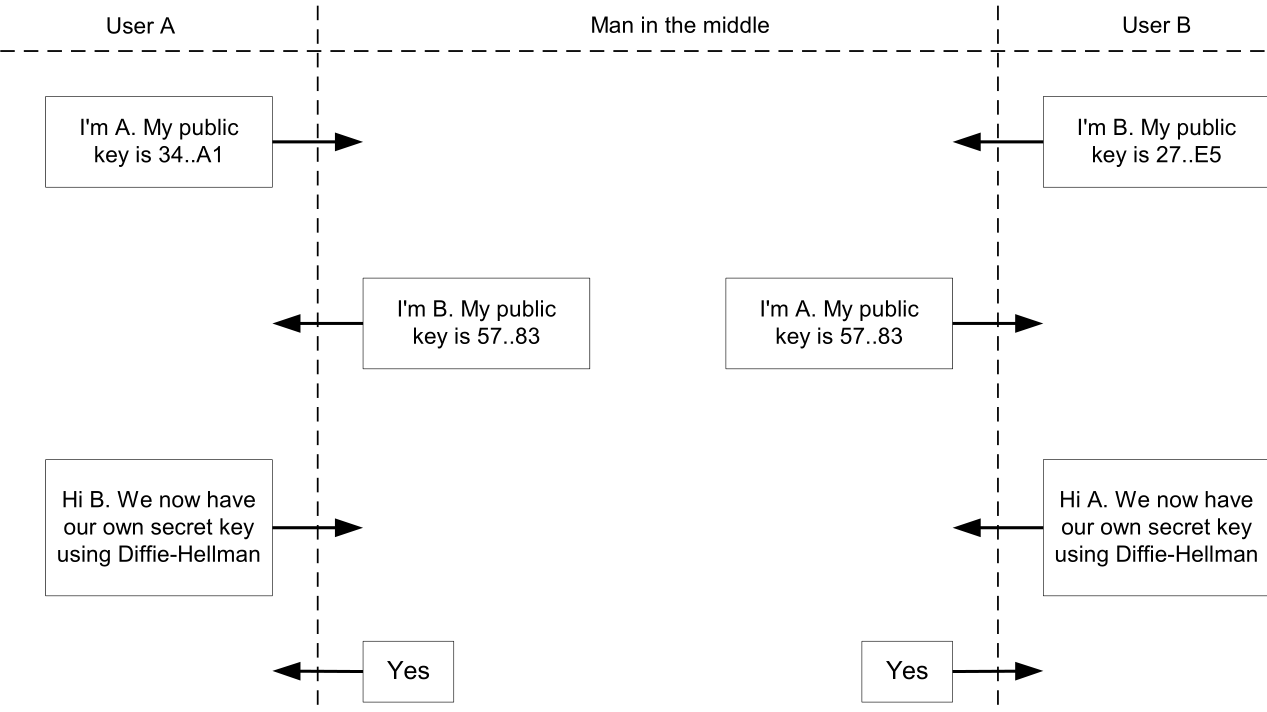
\includegraphics[width=138.60mm,height=196.02mm]{../../images/llm/page_050_img_01.png}%
\end{textblock*}

\end{document}
